%% ----------------------------------------------------------------------------
% CVG SA/MA thesis template
%
% Created 03/08/2024 by Tobias Fischer
%% ----------------------------------------------------------------------------
\newpage
\chapter{Experiments}

% ------- Instructions for writing the experiments section:
% Describe the evaluation you did in a way, such that an independent researcher can repeat it. Cover the following questions:
% \begin{itemize}
 % \item \textit{What is the experimental setup and methodology?} Describe the setting of the experiments and give all the parameters you have used in detail. Give a detailed account of how the experiment was conducted.
 % \item \textit{What are your results?} In this section, a \emph{clear description} of the results is given. If you produced lots of data, include only representative data here and put all results into the appendix. 
% \end{itemize}


\section{Experimental Setup}

\subsection{Datasets}

\paragraph{Hi4D.}
We evaluate on Hi4D, an indoor multi-camera dataset with two interacting people performing complex motions. Hi4D provides multi-view videos as well as ground truth meshes and poses, which enables quantitative evaluation of novel view synthesis, pose estimation, and mesh reconstruction. We follow the evaluation protocol of MultiPly for fair comparison and use the following scenes from Hi4D: \textit{pair15-fight15-view4}, \textit{pair16-jump16-view4}, \textit{pair17-dance17-view28} and \textit{pair19-piggyback19-view4}. Since our estimated cameras and SMPL-X parameters can live in a different world coordinate frame than the ground truth, we apply a camera-based world alignment using the provided camera parameters and use the same alignment consistently across all tasks, including pose and reconstruction metrics.


\paragraph{MMM.}
We also evaluate on MMM \cite{multiply} to cover scenes with more than two people and dynamic camera motion. MMM contains scenes with three to four interacting people captured with a single moving handheld camera and provides ground truth meshes and camera poses, but does not provide the full set of annotations required by all evaluation tasks. Therefore, for MMM we primarily report mesh reconstruction metrics. We follow the evaluation protocol of MultiPly and use the following scenes from MMM: \textit{dance}, \textit{lift} and \textit{walkdance}. 

\subsection{Evaluation Metrics}

\paragraph{Novel view synthesis.}
We evaluate rendering quality using Peak-Signal-to-Noise Ratio (PSNR), Stuctural Similarity Index Measure (SSIM) (higher is better) and Learned Perceptual Image Patch Similarity (LPIPS) (lower is better) \cite{lpips}. PSNR measures the pixel-wise similarity of the reconstructed image by computing the logarithmic ratio between the maximum pixel value and the mean squared error, and is reported in decibels. SSIM measures perceived structural similarity by comparing local luminance, contrast, and structure between images \cite{wikipedia_ssim}. LPIPS is a learned perceptual metric that compares deep features extracted by a pretrained network. And in contrast to the pixel level metrics should be aligned better with the human judgement \cite{lpips}.

For each Hi4D scene, we treat one camera as the source view and evaluate novel view synthesis on the remaining seven cameras. For each target camera and frame, we compute the metrics between the rendered image and the corresponding ground truth image. Following MultiPly, we downscale images by a factor of two for evaluation. We then aggregate the results by averaging over all evaluation frames and all target cameras to obtain a single score per scene. Finally, we report dataset-level results by averaging these per-scene scores.

\paragraph{Pose estimation.}
We assess pose quality using MPJPE (mm) and mean vertex error (MVE, mm), as well as interaction-focused metrics: contact distance (CD, mm) \cite{yin2023hi4d} and percentage of correct depth relations (PCDR) \cite{bev} with a threshold of $0.15$m. Hi4D provides ground truth SMPL parameters, and MultiPly reports pose metrics in the SMPL space. Therefore, for a fair comparison, we convert our predicted SMPL-X parameters to SMPL parameters using the official SMPL-X model transfer procedure \cite{smplx} and evaluate all pose metrics in the SMPL parameterization.

MPJPE measures the mean Euclidean distance between corresponding predicted and ground truth SMPL joints, averaged over all joints and people in the frame, where lower is better. MVE is defined analogously but computes the mean Euclidean distance between corresponding SMPL mesh vertices, and lower values indicate a more accurate reconstruction of the posed body surface. We report MPJPE and MVE in global coordinates and do not apply root alignment.

To capture interaction quality, we report contact distance (CD), which measures how well the predicted meshes reproduce inter-person contact \cite{yin2023hi4d}. Given ground truth contact correspondences between the two SMPL meshes, we compute the average distance between corresponding contact points in the prediction, reported in millimeters, where lower is better. Finally, PCDR measures whether the predicted depth ordering between people matches the ground truth. For each frame, we transform the predicted and ground truth person translations to camera coordinates and derive each person's depth from the $z$ component. We then evaluate all person pairs and check whether their relative depth relation is predicted correctly under the threshold $\tau=0.15$m \cite{bev}. Following the protocol in \cite{bev} used by MultiPly as well, we also group people into ordinal depth layers using a depth-gap threshold $\gamma=0.3$m, and treat pairs within the same layer as being at equal depth. PCDR is reported as the fraction of correctly predicted relations in a frame, where higher is better.


\paragraph{Mesh reconstruction.}
To evaluate geometry, we report volumetric IoU (V-IoU), Chamfer distance (C-$\ell_2$, cm), point-to-surface distance (P2S, cm), and normal consistency (NC). V-IoU measures the overlap between voxelized predicted and ground truth volumes, and higher values indicate better agreement. Chamfer distance measures the average closest-point distance between two point sets sampled from the predicted and ground truth surfaces, and lower values indicate more accurate geometry. P2S measures the average distance from points sampled on the predicted surface to the closest point on the ground truth surface, and lower values indicate better surface accuracy. Normal consistency evaluates agreement between surface orientations by comparing the dot product of predicted normals with the corresponding ground truth normals at nearest surface locations, and higher values indicate more consistent surface orientation.

For this evaluation, we extract meshes from the 3DGS representation using marching cubes. Before we compute the metrics, we align the reconstructed meshes to the ground truth meshes using rigid ICP (no scaling). We run ICP for 10 iterations with a convergence threshold of $10^{-4}$ and use 1000 surface samples to estimate the alignment.

For Chamfer distance, P2S, and normal consistency we estimate the metrics by sampling 1000 points uniformly from each mesh surface. Unfortunately, MultiPly does not report these evaluation hyperparameters, so we choose them ourselves and use the same settings across all methods for fair comparison. For volumetric IoU, we voxelize meshes using voxel size $0.02$ with padding $0.05$ around the joint bounds of predicted and ground truth meshes.

\subsection{Implementation Details}
Unless stated otherwise, we optimize only the 3DGS parameters and keep SMPL-X parameters and camera parameters fixed. We initialize the canonical 3DGS using LHM and apply DiFix to obtain pseudo ground truth novel training views. Each person is represented by $N=40{,}000$ Gaussians.
We optimize the 3DGS parameters using AdamW with learning rate $10^{-4}$ and batch size $5$. We train for 15 epochs and use gsplat \cite{ye2025gsplat} for differentiable Gaussian rendering. To construct the training set, we generate 7 novel training view camera trajectories and subsample the original video frames by a factor of 5 (for example, 100 frames become 20 training timestamps).
For preprocessing, we use the original Hi4D image resolution, while for MMM we downsample images by a factor of 2. For runtime, preprocessing takes roughly 10 to 15 minutes per scene, and training takes roughly 5-10 minutes per scene on a single NVIDIA V100 GPU.

\section{Results}

\subsection{Reconstruction Comparisons}

% selected scene and frames for this qual vis:
% mmm - lift - frame 53
% hi4d pair 19 piggyback - frame 135
\begin{figure}[!ht]
    \centering
    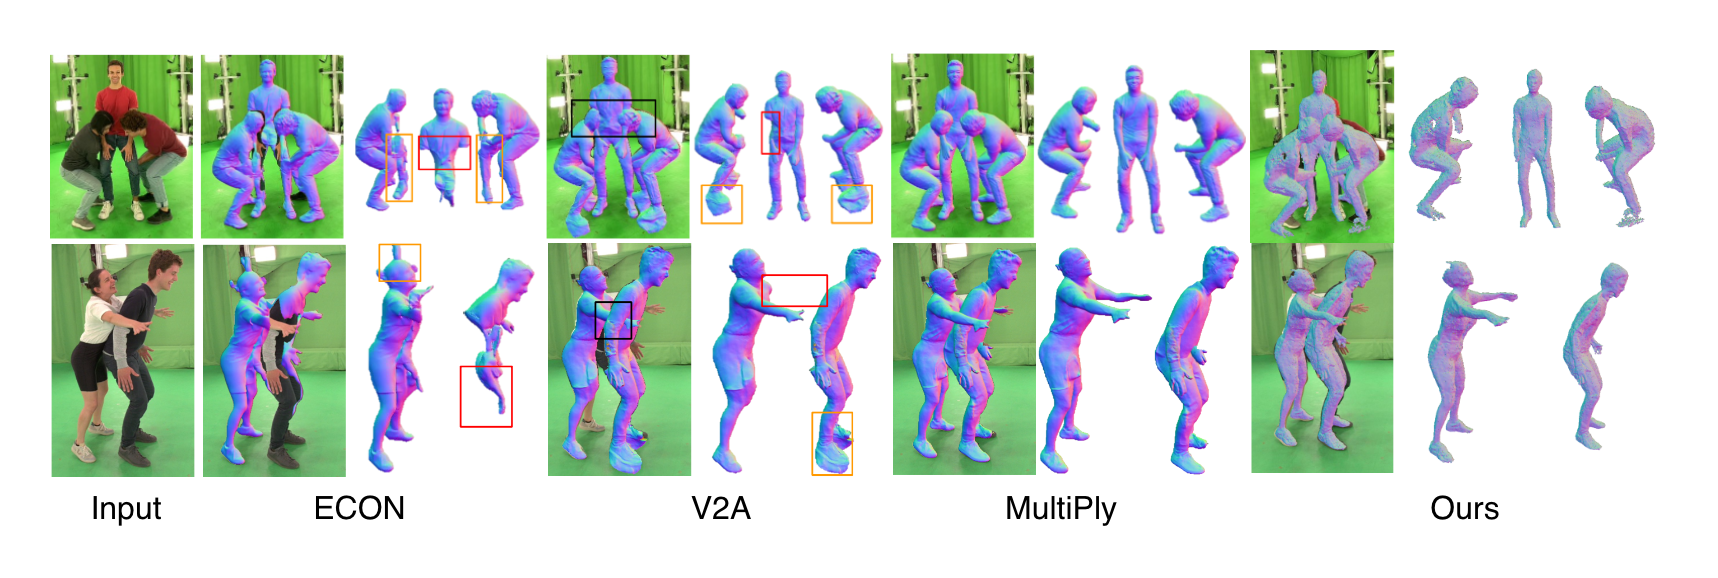
\includegraphics[width=1.0\textwidth]{figures/qual_recon_comp.drawio.png}
    \caption{\textbf{Qualitative reconstruction comparison}. We adopt the figure from MultiPly \cite{multiply} and added our reconstruction results for comparison on chosen scenes from Hi4D and MMM. For each method, we show RGB frame overlaid with a surface normal map. In addition, we also show normal maps for each person separately. The red bounding boxes show missing mesh parts due to occlusion, while the orange bounding boxes highlight extra mesh artifacts caused by poor segmentation.}
    \label{fig:qual_recon_comp}  
\end{figure}

\begin{table}[!ht]
  \centering
  \small
  \setlength{\tabcolsep}{7pt}
  \begin{tabular}{ll
      S[table-format=1.3]
      S[table-format=1.2]
      S[table-format=1.2]
      S[table-format=1.3]}
    \toprule
    \textbf{Dataset} & \textbf{Method} & \multicolumn{1}{c}{\textbf{V-IoU} $\uparrow$} & \multicolumn{1}{c}{\textbf{C-$\ell_2$} $\downarrow$} & \multicolumn{1}{c}{\textbf{P2S} $\downarrow$} & \multicolumn{1}{c}{\textbf{NC} $\uparrow$} \\
    \midrule
    Hi4D & ECON & 0.787 & 3.72 & 3.59 & 0.746 \\
     & V2A & 0.783 & 3.02 & 2.46 & 0.775 \\
     & MultiPly & \textbf{0.816} & \textbf{2.53} & \textbf{2.34} & \textbf{0.789} \\
     & Ours & 0.560 & 4.63 & 2.86 & 0.733 \\
    \midrule
    MMM & ECON & 0.760 & 4.17 & 3.71 & 0.705 \\
     & V2A & 0.812 & 3.34 & 2.68 & 0.735 \\
     & MultiPly & \textbf{0.826} & \textbf{2.89} & \textbf{2.40} & \textbf{0.757} \\
     & Ours & 0.377 & 6.33 & 3.86 & 0.641 \\
    \bottomrule
  \end{tabular}
  \caption{\textbf{Human mesh reconstruction results on Hi4D and MMM.} Best results per dataset and metric are in bold.}
  \label{tab:reconstruction_results}
\end{table}

We compare our mesh reconstruction quality to MultiPly \cite{multiply} and additionally report ECON \cite{econ} and Vid2Avatar (V2A) \cite{guo2023vid2avatar} as reference baselines used in MultiPly. As Table \ref{tab:reconstruction_results} shows, across both Hi4D and MMM, MultiPly achieves the best scores across all reconstruction metrics, while our method trails and degrades further on MMM, which contains more people and dynamic camera motion. We attribute the gap mainly to two factors: first, errors in the fixed pose initialization can place the posed 3DGS in an incorrect configuration, which directly hurts volume and surface metrics; second, MultiPly reconstructs an implicit signed distance field that is designed for surface extraction, whereas our explicit 3DGS is optimized for rendering and mesh extraction via marching cubes on a density field is only an approximation. Overall, these results suggest that the current pipeline is not yet competitive for high-fidelity geometry, and that improving pose refinement and surface extraction is the most direct direction for future work.

Figure \ref{fig:qual_recon_comp} is consistent with the quantitative reconstruction results. Our method typically recovers the coarse body geometry and, in the shown examples, avoids severe missing-body artifacts under occlusion (red boxes). However, fine surface details are often smoothed out, and the extracted meshes can exhibit blobby, bubble-like artifacts, which we attribute to extracting a surface from a rendering-optimized Gaussian density field rather than directly optimizing a watertight surface representation. In the upper row, we additionally observe spurious geometry around the right person's left foot.


\subsection{Pose Estimation Comparisons}

% selected scene and frames for this qual vis:
%  Pair15 - frame 87, Pai19 - frame 132

\begin{figure}[!ht]
    \centering
    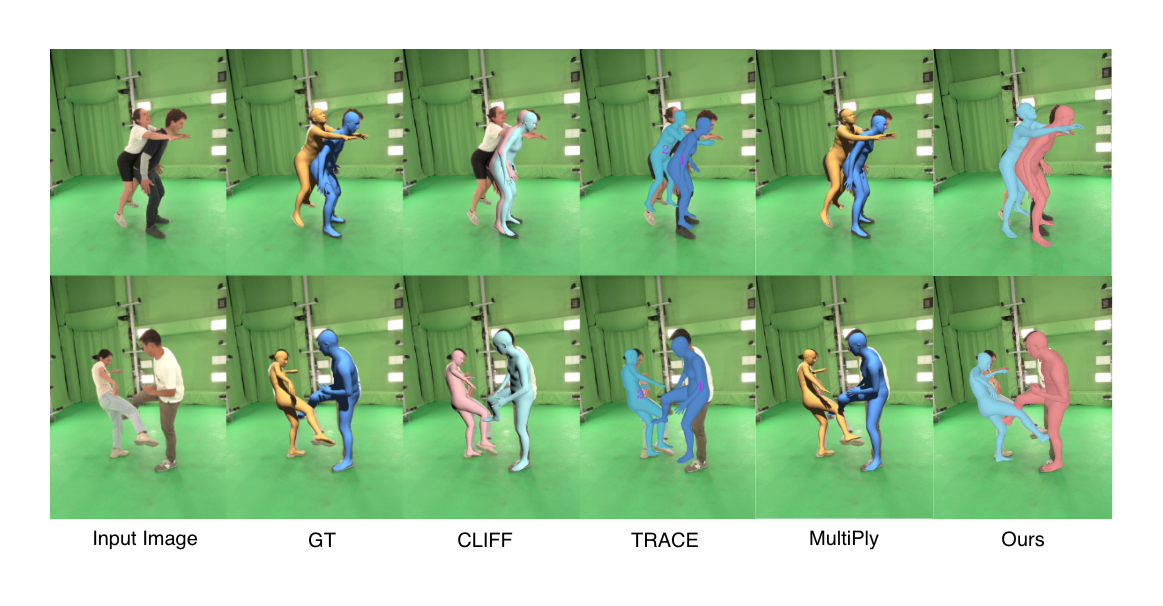
\includegraphics[width=1.0\textwidth]{figures/qual_pose_comp.drawio.png}
    \caption{\textbf{Qualitative pose estimation comparison}. We adopt the figure from MultiPly \cite{multiply} and added our pose estimation results for comparison on chosen scenes from Hi4D. For each method, we show RGB frame overlaid with predicted SMPL-(X) mesh.}
    \label{fig:qual_pose_comp}  
\end{figure}

\begin{table}[!ht]
  \centering
  \small
  \setlength{\tabcolsep}{6pt}
  \begin{tabular}{l
      S[table-format=2.1]
      S[table-format=3.1]
      S[table-format=3.1]
      S[table-format=1.3]}
    \toprule
    \textbf{Method} & \multicolumn{1}{c}{\textbf{MPJPE} $\downarrow$} & \multicolumn{1}{c}{\textbf{MVE} $\downarrow$} & \multicolumn{1}{c}{\textbf{CD} $\downarrow$} & \multicolumn{1}{c}{\textbf{PCDR} $\uparrow$} \\
    \midrule
    CLIFF & 85.7 & 102.1 & 351.7 & 0.606 \\
    TRACE & 95.6 & 115.7 & 249.4 & 0.603 \\
    MultiPly & \textbf{69.4} & 83.6 & 218.4 & \textbf{0.709} \\
    Ours (using Human3R) & 93.9 & \textbf{77.7} & \textbf{195.8} & 0.647 \\
    \bottomrule
  \end{tabular}
  \caption{\textbf{Human pose estimation results on Hi4D.} Best results are in bold.}
  \label{tab:pose_results_hi4d}
\end{table}

We compare our pose estimation results to MultiPly \cite{multiply} and include for reference CLIFF \cite{li2022cliff} and TRACE \cite{trace} as reported by MultiPly. MultiPly initializes poses with TRACE, refines them using ViTPose \cite{vitpose}, and further optimizes poses during training via a photometric loss, while our method relies on the initial Human3R estimates \cite{chen2025human3r} without refinement. The quantiative results in Table \ref{tab:pose_results_hi4d} show a clear trade-off: MultiPly achieves the best MPJPE and PCDR, indicating more accurate joint locations and depth ordering, while our method achieves lower MVE and CD, indicating smaller vertex-space error and closer inter-person contact distances. A likely reason is that we keep pose fixed and do not apply 2D keypoint refinement or pose optimization during training, so residual global pose errors remain and affect joint-based metrics, while surface-based metrics can still benefit from the SMPL prior and the fixed interaction configuration. Overall, the pose results suggest that adding pose refinement and optimization is the most direct path to improve MPJPE and PCDR without sacrificing the strong contact behavior.

Figure \ref{fig:qual_pose_comp} illustrates that, compared to MultiPly, our method can exhibit a small misalignment between the RGB frame and the rendered SMPL-X mesh. We attribute this misalignment primarily to the lack of an explicit 2D keypoint-based pose refinement stage (e.g., ViTPose) as used in MultiPly. Nevertheless, the bottom-row example also highlights a practical advantage of using SMPL-X rather than SMPL: the subject's right-hand articulation is better captured by our SMPL-X-based predictions, whereas MultiPly's SMPL-based fit results in a more neutral hand pose.

\subsection{Instance Segmentation Comparisons}
Qualitative and quantitative instance segmentation comparisons are included in Appendix~\ref{sec:appendix_segmentation}.

\subsection{Novel View Synthesis Comparisons}

% selected scene and frames for this qual vis:
% Pair 16 - frame 66, Pair 15 - frame 90
\begin{figure}[!ht]
    \centering
    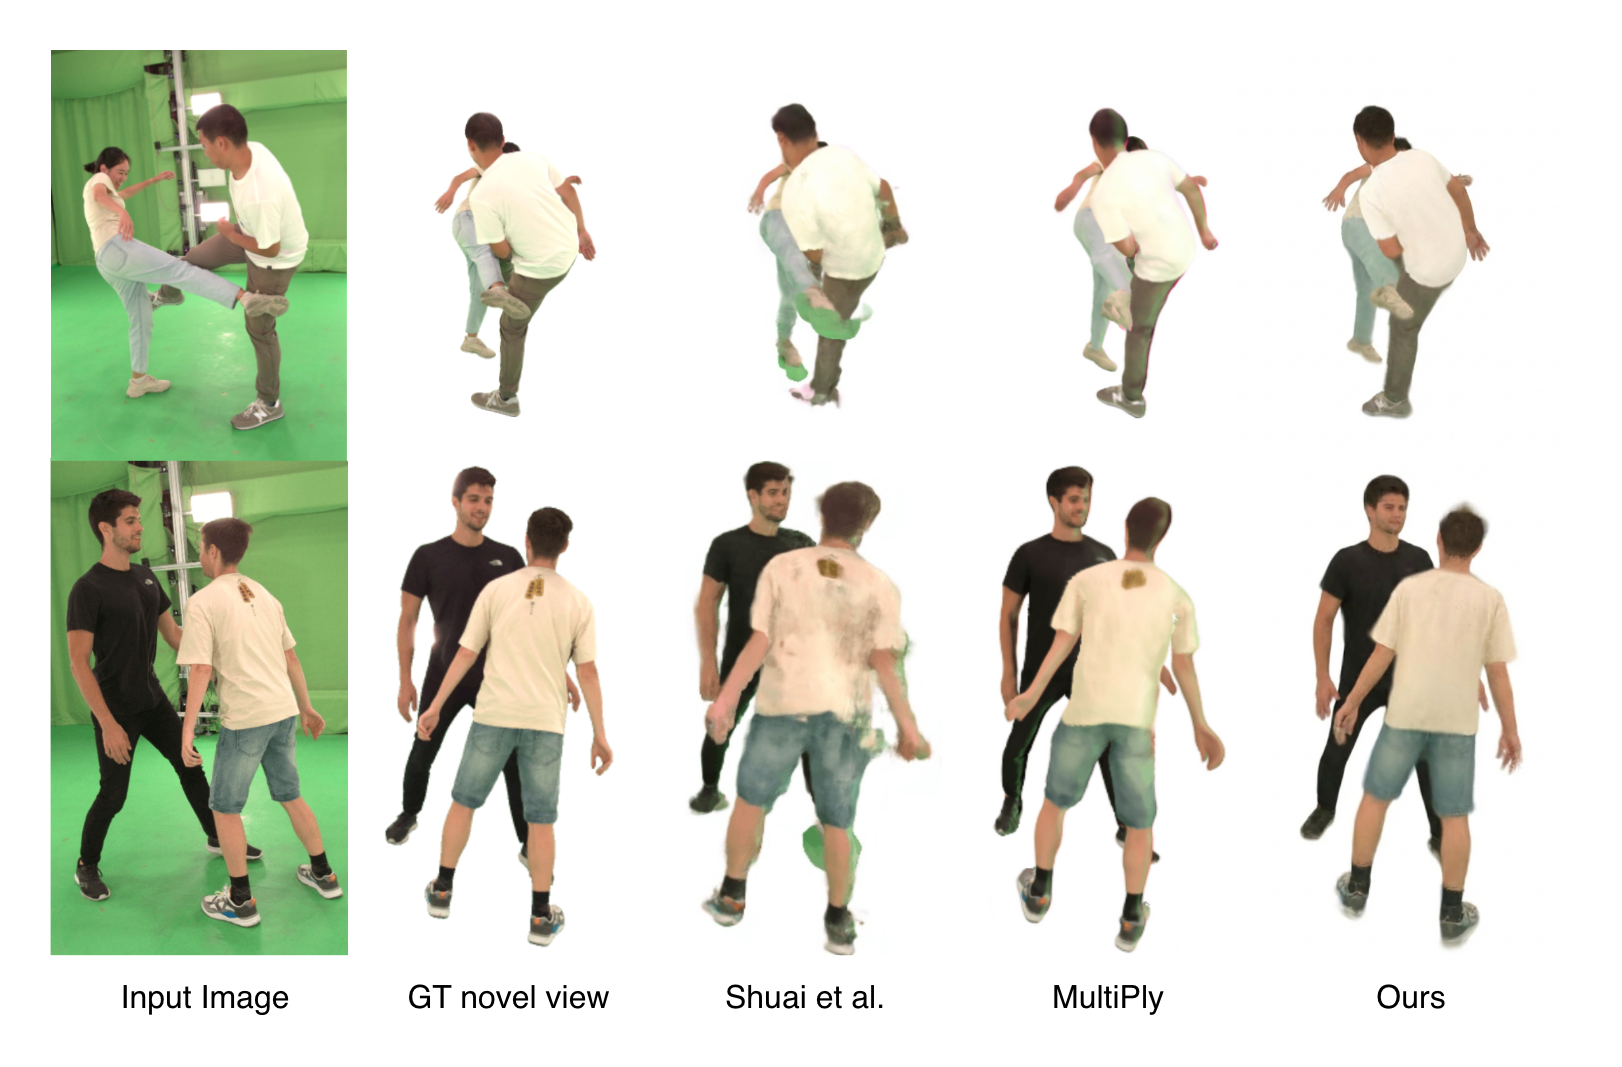
\includegraphics[width=1.0\textwidth]{figures/qual_nvs_comp.drawio.png}
    \caption{\textbf{Qualitative novel view synthesis comparison}. We adapt the figure from MultiPly \cite{multiply} and show the original source camera view along with the ground truth novel view and predictions from our method and relevant baselines.}
    \label{fig:qual_nvs_comp}  
\end{figure}

\begin{table}[!ht]
  \centering
  \small
  \setlength{\tabcolsep}{7pt}
  \begin{tabular}{l
      S[table-format=1.3]
      S[table-format=2.1]
      S[table-format=1.4]}
    \toprule
    \textbf{Method} & \multicolumn{1}{c}{\textbf{SSIM} $\uparrow$} & \multicolumn{1}{c}{\textbf{PSNR} $\uparrow$} & \multicolumn{1}{c}{\textbf{LPIPS} $\downarrow$} \\
    \midrule
    Shuai et al. & 0.898 & 19.6 & 0.1099 \\
    MultiPly & 0.915 & \textbf{20.7} & \textbf{0.0798} \\
    Ours & \textbf{0.926} & 20.2 & 0.0872 \\
    \bottomrule
  \end{tabular}
  \caption{\textbf{Novel view synthesis results on Hi4D.} Best results are in bold.}
  \label{tab:nvs_results_hi4d}
\end{table}


In addition to MultiPly, we also compare to Shuai et al. \cite{nv_interact}, a multi-view method that was adapted by MultiPly to work in a monocular setting. Under the masked, downscaled evaluation protocol described above, our method achieves the best SSIM, while MultiPly achieves the best PSNR and LPIPS. This indicates that our renderings better preserve global structure, while MultiPly retains more pixel-level detail and perceptual fidelity. Overall, our novel view synthesis quality is competitive in terms of structural similarity, but there remains a gap in fine details compared to MultiPly.

Figure \ref{fig:qual_nvs_comp} provides qualitative novel view synthesis comparisons. In the bottom-row example, our method preserves the head shape of the subject closer to the camera and produces sharper local details than MultiPly. This sharpening may partially explain why our PSNR is slightly lower, as PSNR is sensitive to pixel-wise differences even when images appear perceptually crisp. At the same time, MultiPly better preserves the tag on the back of the subject, which we attribute to our initialization: since LHM observes the person from essentially a single view, details that are never visible (such as a back-facing tag) may not be reconstructed reliably and therefore cannot be reinforced through backpropagation during training. Finally, in the top-row example, MultiPly exhibits greenish color artifacts that are likely caused by background pixels leaking into the foreground during progressive mask refinement. We do not observe these artifacts in our renderings, which we attribute to refining synthesized training views with DiFix, helping to suppress such mask-related color leakage.


\subsection{Ablation Studies}

\paragraph{Novel Training View Synthesis.}

\begin{table}[!ht]
  \centering
  \small
  \setlength{\tabcolsep}{7pt}
  \begin{tabular}{c
      c
      l
      S[table-format=1.3]
      S[table-format=2.1]
      S[table-format=1.4]}
    \toprule
    \textbf{LHM Init} & \textbf{DiFix} & \textbf{Reference Camera} & \multicolumn{1}{c}{\textbf{SSIM} $\uparrow$} & \multicolumn{1}{c}{\textbf{PSNR} $\uparrow$} & \multicolumn{1}{c}{\textbf{LPIPS} $\downarrow$} \\
    \midrule
    $\checkmark$ & $\times$ & - & 0.925 & 20.0 & \textbf{0.0818} \\
    \midrule
    $\times$ & $\times$ & - & 0.890 & 17.0 & 0.1343 \\
    $\times$ & $\checkmark$ & Source & 0.903 & 17.1 & 0.1184 \\
    $\times$ & $\checkmark$ & Previous & 0.900 & 17.0 & 0.1206 \\
    $\checkmark$ & $\checkmark$ & Source & \textbf{0.926} & \textbf{20.2} & 0.0865 \\
    $\checkmark$ & $\checkmark$ & Previous & \textbf{0.926} & \textbf{20.2} & 0.0872 \\
    \bottomrule
  \end{tabular}
  \caption{\textbf{Ablation study on novel view synthesis.} Results are reported under the same evaluation protocol as Table~\ref{tab:nvs_results_hi4d}. The \textbf{LHM Init} and \textbf{DiFix} columns indicate whether the corresponding component is enabled. Best results are in bold.}
  \label{tab:ablation_nvs}
\end{table}

\noindent Table~\ref{tab:ablation_nvs} isolates the impact of (i) LHM initialization, (ii) DiFix-based refinement of synthesized novel training views, and (iii) the choice of reference camera for DiFix (source view versus the previously synthesized view). Training without LHM initialization and without any view synthesis performs worst, highlighting that learning a renderable representation from strictly monocular supervision is challenging under our compute budget. Adding novel training views that are rendered from the partially trained model and refined with DiFix yields only a modest improvement in this setting.

\noindent LHM initialization is the dominant factor: simply initializing from LHM (without DiFix) substantially improves all metrics and provides the best LPIPS in our ablation. Adding DiFix refinement on top of LHM leads to only marginal changes: SSIM and PSNR improve slightly, while LPIPS becomes worse. Figure~\ref{fig:qual_difix_comp} provides an explanation for this behavior. Without LHM initialization, the intermediate renders are substantially degraded, which gives DiFix too much freedom during refinement; in both reference strategies, this leads to implausible hallucinations, such as an incorrect rotation of the head. With LHM initialization, the renders are already significantly closer to the target view, and DiFix mainly acts as a detail enhancement module, sharpening local texture without correcting higher-level geometric errors. Finally, using the source camera versus the previous synthesized camera as the DiFix reference yields very similar results, with a slight advantage for the source-reference strategy, suggesting that potential error accumulation in the chained (previous-reference) strategy can offset the benefit of higher overlap. Despite the small advantage of the source-reference strategy in this ablation, we use the previous-reference strategy in our main pipeline, as we expect it to benefit more from the higher inter-view overlap when the refinement model is stronger and produces less drift.

\begin{figure}[!ht]
    \centering
    \includegraphics[width=0.9\textwidth]{figures/qual_difix_comp.drawio.png}
    \caption{\textbf{Qualitative comparison of novel training view synthesis}. We show comparison of novel view synthesis strategies along the following axis: (i) LHM initialization vs. random initialization, and (ii) DiFix refinement using source view vs. previous view. In total, we show four possible configurations. In each configuration, we show the reference view (left column), the rendered view to be refined (middle column), and the refined view by DiFix (right column).}
    \label{fig:qual_difix_comp}  
\end{figure}

\begin{figure}[!ht]
    \centering
    \includegraphics[width=0.8\textwidth]{figures/n_trn_cameras_ablation_setup.drawio.png}
    \caption{\textbf{Distribution of the cameras for the ablation}. We show the distribution of the cameras used in the ablation study on the number of novel training cameras. The blue camera is the source camera, the orange cameras are the novel training cameras. Specifially, we experiment with 0, 2, 4, and 7 novel training cameras.}
    \label{fig:n_trn_cameras_ablation_setup}  
\end{figure}


% We will skip this for now since it adds little value compared to the table and the other fig
% \begin{figure}[!ht]
    % \centering
    % \includegraphics[width=1.0\textwidth]{figures/qual_diff_trn_nv_strategies.drawio.png}
    % \caption{\textbf{Qualitative comparison of synthesised novel views based on different novel view training strategies}. First row: no training novel cameras synthesised, novel training cameras synthesised using either source or previous camera as reference. Second row: synthesised view of the LHM initialized 3DGS, novel training cameras synthesised using either source or previous camera as reference.}
    % \label{fig:qual_comp_trn_nvs_strategies}  
% \end{figure}


\paragraph{Number of training cameras.}

\begin{table}[!ht]
  \centering
  \small
  \setlength{\tabcolsep}{7pt}
  \begin{tabular}{c
      S[table-format=1.3]
      S[table-format=2.1]
      S[table-format=1.4]}
    \toprule
    \textbf{Number of Novel Training Cameras} & \multicolumn{1}{c}{\textbf{SSIM} $\uparrow$} & \multicolumn{1}{c}{\textbf{PSNR} $\uparrow$} & \multicolumn{1}{c}{\textbf{LPIPS} $\downarrow$} \\
    \midrule
    0 & 0.908 & 18.8 & 0.1134 \\
    2 & 0.922 & 20.1 & 0.0953 \\
    4 & 0.925 & \textbf{20.3} & 0.0903 \\
    7 & \textbf{0.926} & 20.2 & \textbf{0.0872} \\
    \bottomrule
  \end{tabular}
  \caption{\textbf{Ablation study on number of novel training cameras}. Best results are in bold.}
  \label{tab:ablation_num_trn_cams}
\end{table}

One motivation for introducing DiFix-based novel training view synthesis is that optimizing a 3DGS model from monocular video requires multi-view supervision. Without additional views, we expect poor novel view synthesis performance, even when starting from an LHM initialization, because subsequent monocular fine-tuning can overfit to the single source view. To test this assumption, we ablate the number of novel training cameras used during training. We consider 0, 2, 4, and 7 novel training cameras, where 0 means training uses only the source camera. All experiments are initialized from LHM; when novel cameras are used, their training images are synthesized and refined with DiFix. Figure~\ref{fig:n_trn_cameras_ablation_setup} shows the camera distribution used in this ablation.

Table~\ref{tab:ablation_num_trn_cams} confirms this hypothesis. Using 0 novel training cameras performs substantially worse across all metrics, indicating that monocular fine-tuning alone is insufficient despite the strong LHM initialization. Adding just 2 novel training cameras yields a large improvement, while increasing from 2 to 4 and 7 yields diminishing returns. Overall, 7 cameras achieves the best SSIM and LPIPS, while PSNR peaks at 4 cameras with a small difference to 7. Despite these diminishing returns, we decided to use 7 novel training cameras in our main pipeline to maximize multi-view supervision during training.

